\section{Introducción}

\subsection{Marco contextual}

\begin{frame}{Caja}
  \begin{Block}{Nombre de la caja}
    Caja verde:
    \begin{itemize}
      \item Definiciones
      \item Constraste con caja azul
    \end{itemize}
  \end{Block}
  \begin{BlueBlock}{Nombre de la caja}
    Caja azul:
    \begin{itemize}
      \Bitem Información a resaltar que no sea una definición
      \Bitem Constrate con una caja verde
    \end{itemize}
  \end{BlueBlock}
  \begin{AlertBlock}{Nombre de la caja}
    Caja naranja par hacer preguntas
  \end{AlertBlock} 
\end{frame}

\begin{frame}{Dos columnas}
  \begin{twocols}
    \colx{
      \begin{itemize}
        \item item
        \item item
      \end{itemize}
    }
    \coly{
      \centering
      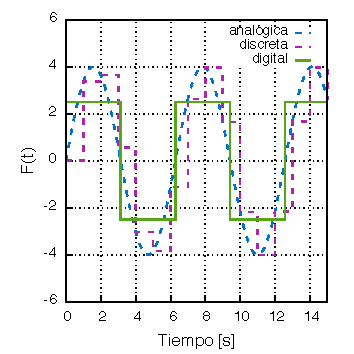
\includegraphics[width = \textwidth]{analog}
    }
  \end{twocols}
\end{frame}

\begin{frame}{Definición única}
  \centering
  \begin{singledef}{Definición}
    Esta es una definición única
  \end{singledef}
\end{frame}
%--- Next Frame ---%


